\documentclass[10pt,a4paper]{article}
\usepackage[utf8]{inputenc}

\usepackage[landscape,margin=1cm]{geometry}
\usepackage[english]{babel}


% colour themes to come. KnitR?

%-------------------------

\title{\color{alert} Cheatsheet:\\ 
{\color{black} protocol Perpetual Swaps}}
\author{Vasili Serchev\\vasili.serchev@protonmail.com}
\date{Dec, 2021}
\usepackage[default]{raleway}
\usepackage{fontawesome}
\usepackage[T1]{fontenc}

\usepackage{hyperref}
\usepackage{enumitem}
\usepackage{lipsum}

\usepackage{xcolor}
\definecolor{customcolor}{HTML}{4c524d}
\definecolor{alert}{HTML}{CD5C5C}
\definecolor{blue}{HTML}{4DA6FF}
\definecolor{mygreen}{HTML}{417d65}
\definecolor{formulacolor}{HTML}{3E8050}
\definecolor{w3schools}{HTML}{4CAF50}
\definecolor{subbox}{gray}{0.60}
\definecolor{codecolor}{HTML}{FFC300}
\colorlet{xx}{customcolor}


%--------------------------Editor mode.

\usepackage
[citestyle=authoryear,
sorting=nty,	  		%Sorts bibliography by year, name, title
autocite=footnote, 		%Autocite command generates footnotes
autolang=hyphen, 		
mincrossrefs=1, 	
backend=biber]
{biblatex}

\DeclareFieldFormat{postnote}{#1}
\DeclareFieldFormat{multipostnote}{#1}
\DeclareAutoCiteCommand{footnote}[f]{\footcite}{\footcites}

\bibliography{literature}
%----------------------------------------
%--------------------------------------------------------------------------------
\usepackage{tcolorbox}

\tcbuselibrary{most,listingsutf8,minted}

\tcbset{tcbox width=auto,left=1mm,top=1mm,bottom=1mm,
right=1mm,boxsep=1mm,middle=1pt}

\newenvironment{mycolorbox}[2]{%
\begin{tcolorbox}[grow to left by=-1em,grow to right by=-1em,capture=minipage,fonttitle=\large\bfseries, enhanced jigsaw,boxsep=1mm,colback=#1!30!white,on line,tcbox width=auto, toptitle=0mm,colframe=#1,opacityback=0.7,nobeforeafter,title=#2]%
}{\end{tcolorbox}\\[0.2em]}

\newenvironment{subbox}[2]{%
\begin{tcolorbox}[capture=minipage,fonttitle=\normalsize\bfseries, enhanced jigsaw,boxsep=1mm,colback=#1!30!white,on line,tcbox width=auto,left=0.3em,top=1mm, toptitle=0mm,colframe=#1,opacityback=0.7,nobeforeafter,title=#2]\footnotesize %
}{\normalsize\end{tcolorbox}\vspace{0.1em}}

\newenvironment{multibox}[1]{%
\begin{tcbraster}[raster columns=#1,raster equal height,nobeforeafter,raster column skip=1em,raster left skip=1em,raster right skip=1em]}{\end{tcbraster}}

\newenvironment{textbox}[1]{\begin{mycolorbox}{customcolor}{#1}}{\end{mycolorbox}}

%-------------------------------
\newtcblisting{codebox}[2]{colback=codecolor!5,colframe=codecolor!80!black,listing only, 
minted options={numbers=left,style=tcblatex,fontsize=\tiny,breaklines,autogobble,linenos,numbersep=3mm},
left=5mm,enhanced,
title=#2, fonttitle=\bfseries,
listing engine=minted,minted language=#1}

%--------------------------------------------------------------------------------
\newcommand{\punkti}{~\lbrack\dots\rbrack~}

\renewenvironment{quote}
               {\list{\faQuoteLeft\phantom{ }}{\rightmargin\leftmargin}%
                \item\relax\scriptsize\ignorespaces}
               {\unskip\unskip\phantom{xx}\faQuoteRight\endlist}
               

%--------------------------------------------------------------------------------
\newcommand{\bgupper}[3]{\colorbox{#1}{\color{#2}\huge\bfseries\MakeUppercase{#3}}}
\newcommand{\bg}[3]{\colorbox{#1}{\bfseries\color{#2}#3}}

\newcommand{\mycommand}[2]{{\ttfamily\detokenize{#1}}~\dotfill{}~{\footnotesize #2}\\}
\newcommand{\sep}{{\scriptsize~\faCircle{ }~}}


\newcommand{\bggreen}[1]{\medskip\bgupper{w3schools}{black}{#1}\\[0.5em]}
\newcommand{\green}[1]{\smallskip\bg{mygreen}{white}{#1}}
\newcommand{\red}[1]{\smallskip\bg{alert}{white}{#1}}
\newcommand{\blue}[1]{\smallskip\bg{blue}{white}{#1}}
\newcommand{\formula}[1]{\smallskip\bg{formulacolor}{white}{#1}}

\usepackage{multicol}
\setlength{\columnsep}{30pt}

\setlength{\parindent}{0pt}
\pagestyle{empty}

\usepackage{csquotes}

\newcommand{\loremipsum}{Lorem ipsum dolor sit amet.}



%--------------------------------------------------------------------------------
\begin{document}
\small
\begin{multicols}{3}

\maketitle
\thispagestyle{empty}
\scriptsize
\tableofcontents


\section{Overview}
\begin{textbox}{Perpetual Swaps in a nutshell}
A perpetual swap allows traders to go long or short a currency pair (e.g., BTCUSD).
\begin{itemize}
\item \textbf{Leveraged trades}: The trader deposits a margin that can be smaller than the notional amount traded
\item There is no expiry of a perpetual swap. The trader can increase, decrease, or exit the position at any time
\item If the value of the position falls below a threshold (=\textbf{maintenance margin})
before the trader closes the position, the position is liquidated
\item Perpetuals feature \textbf{funding payments}. These payments have been introduced to keep the Perpetual price as 
close as possible to the underlying spot index price.
If the Perpetual trades at a higher price than the index, traders that have long positions need to make funding payments 
to the traders with short positions. 
This will make the product less attractive to the long position holders and more attractive to the short position holders. 
This will cause the Perpetuals price 
to trade in line with the price of the index. If the Perpetual trades at a price lower than the index, the short position holders 
will have to pay the long position holders. Funding rates are quoted per 8 hours (e.g. 0.0001\% per
8h) and are paid continuously
\end{itemize}
\end{textbox}


\begin{textbox}{Mark Price and Funding Rate}
The \textbf{Mark Premium Rate}, $\bar{r}$, is an exponentially weighted moving average of the
relative deviation of the mid-price to the spot index.
The  \textbf{Funding Rate} is a function of this rate:
\begin{align}
    f= \max\left[ \bar{r}, \Delta\right] +
    \min\left[ \bar{r}, -\Delta\right] +
    \text{sgn}(-k^\star)  0.01\%,
\end{align}
where $-k^\star$ is the trade size that brings the AMM to its minimal risk.
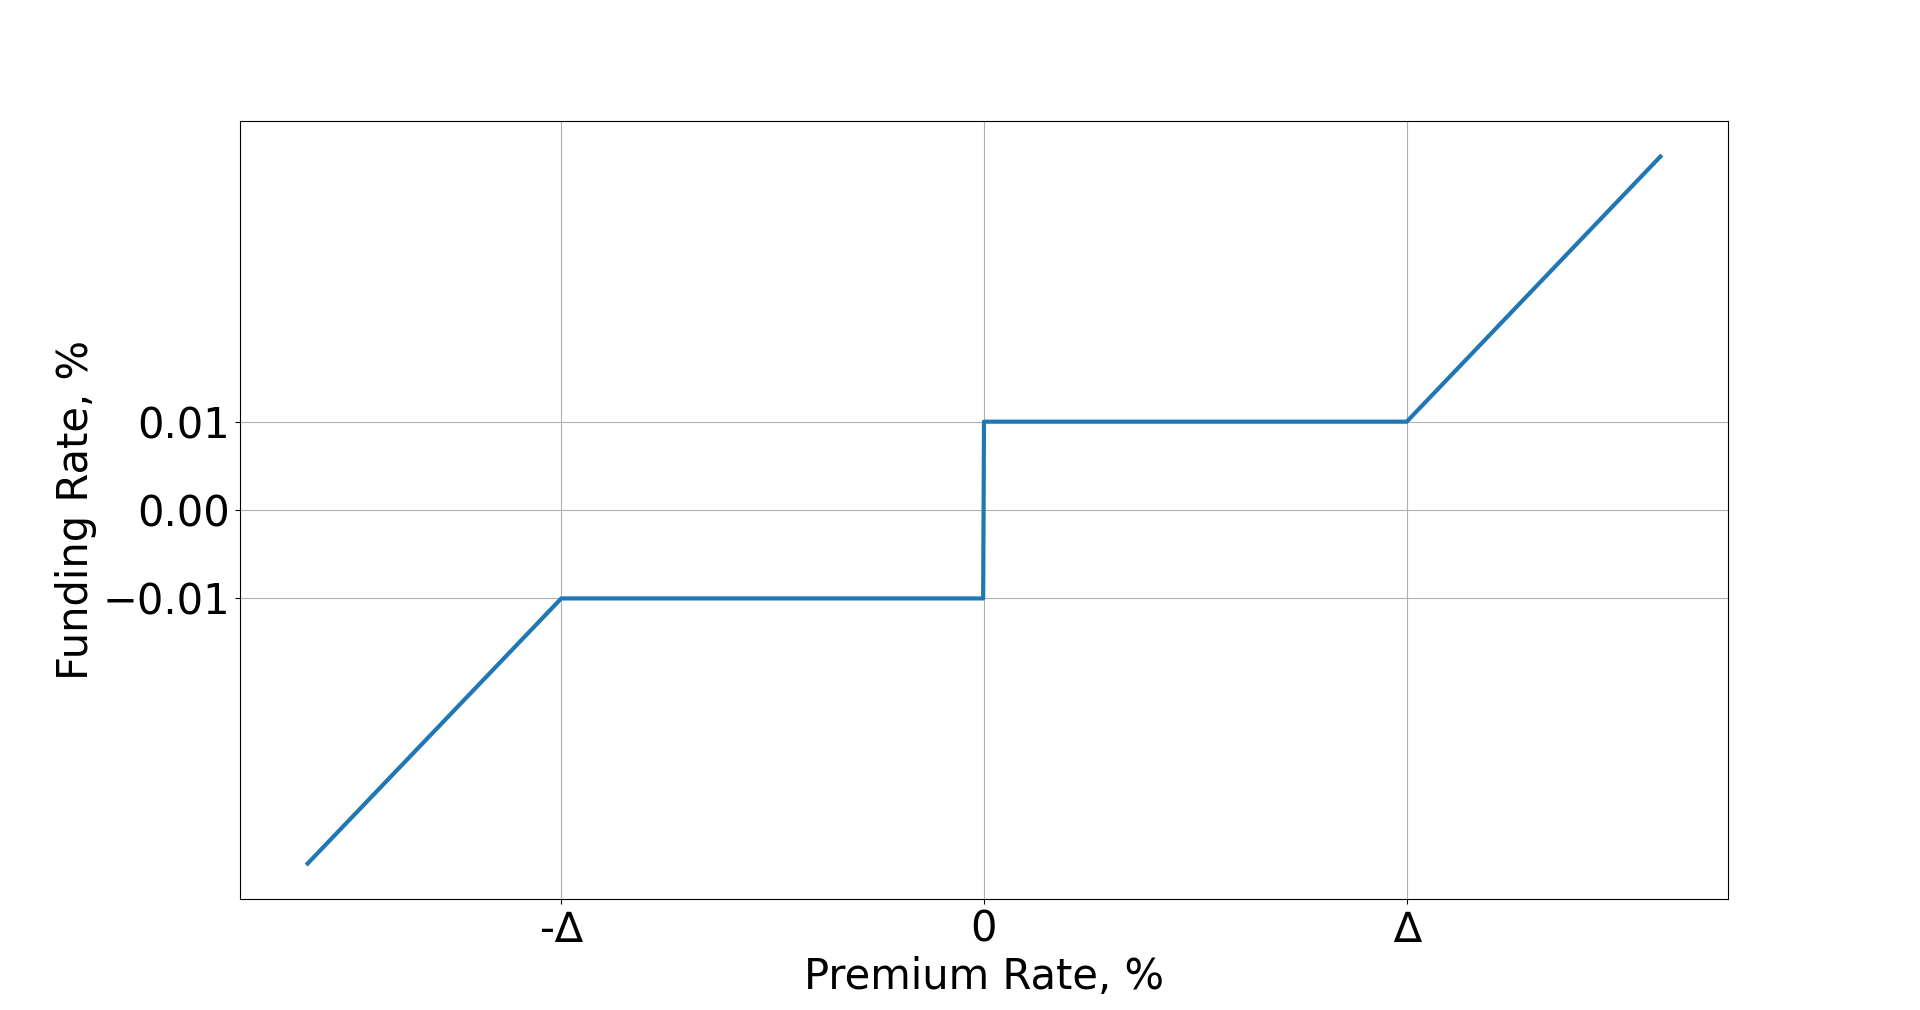
\includegraphics[width=\textwidth]{fundingrate.png}\\
There is a \textbf{cap} on the Funding Rate to ensure the maximum 
leverage can still be utilized. The absolute Funding Rate is capped at 90\% of 
Initial Margin - Maintenance Margin.

The \textbf{Mark Price} is the Mark Premium rate applied to the Spot Index $s_2$:
\begin{align}
    \bar{s}_2 = s_2 (1+\bar{r}).
\end{align}
\end{textbox}

\begin{textbox}{AMM}
protocol perpetuals use an \textbf{automated market maker} (AMM) to determine
the Perpetual Swap price. 
\begin{itemize}
\item The counterparty for each trade is the AMM
\item The AMM holds margin collateral like a trader. in Addition,
the AMM holds \textbf{liquidity reserves}, an AMM fund for each perpetual, and
a shared default fund
\item If the aggregated long trader position equals the (absolute) aggregated short
trader position, a price move will not change the AMM reserve balances. 
In contrast, a non-zero net aggregated position exposes the AMM to market risk
\item The perpetual \textbf{price} exceeds the underlying spot price if there is excess
demand for the long side. The price is below spot if there is excess demand for the short
\item \textbf{Funding rates} depend on the deviation of the perpetual price from the 
underlying spot price
\item This \textbf{pricing method
incentivizes traders to minimize the AMM risk}
\end{itemize}
\end{textbox}

\begin{textbox}{Currencies}
	{\red{Base Currency}\green{Quote Currency}-\blue{Collateral Currency}}\\
	\textbf{\color{red}{The position size is denoted in Base Currency.}} 
	\textbf{\color{mygreen}{The price of the perpetual per unit of base currency is quoted
	in Quote Currency}} 	
	\textbf{\color{blue}{The trader margin is deposited in collateral currency. Profit and
	loss are paid in collateral currency.}} 
	\begin{enumerate}
	    \item \textbf{\color{red}{BTC}\color{mygreen}{USD} - \color{blue}{BTC}} \\
	    Trade BTC quoted in USD (e.g., \$40,000 per BTC) with margin collateral in BTC
	    \item \textbf{\color{red}{BTC}\color{mygreen}{XUSD} - \color{blue}{XUSD}} \\
	    Trade BTC quoted in USD (e.g., \$40,000 per BTC) with margin collateral in XUSD
	    \item \textbf{\color{red}{ETH}\color{mygreen}{BTC} - \color{blue}{BTC}} \\
	    Trade ETH quoted in BTC (e.g., 0.07 BTC per ETH) with margin collateral in BTC
	     \item \textbf{\color{red}{ETH}\color{mygreen}{USD} - \color{blue}{BTC}} \\
	    Trade ETH quoted in USD (e.g., \$4000 per BNB) with margin collateral in XUSD
	\end{enumerate}
	If the collateral currency is different from the 
	base currency and the quote currency, we call the instrument a \textbf{quanto perpetual}.
	The \textbf{AMM} design supports any combination of base, quote, and collateral currency.
	Perpetual Swaps with the same collateral currency can share a \emph{liquidity pool}.
\end{textbox}

\begin{textbox}{Liquidity Pools}
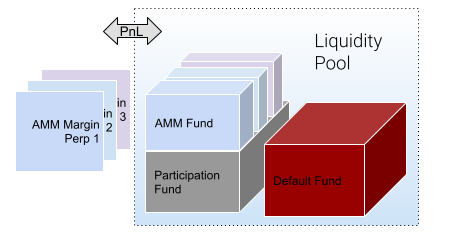
\includegraphics[width=\textwidth]{CapitalPots.png}
Perpetuals with the same 
    collateral currency can share one 'liquidity pool', consisting of
    an AMM fund (a capital reserve set up for each perpetual),
    a participation fund built up by external PnL participants, and a default fund.
    The Profit \& Loss ('PnL') of the AMM is regularly exchanged 
    with the liquidity pool so that the AMM margin balance 
    corresponds to the initial margin. That is,
    losses are covered with funds  
    from the liquidity pool, and profits above the initial margin rate
    are sent to the pool.
\end{textbox}

\begin{textbox}{Margin Terminology}
The collateral required to trade is determined by the
\emph{initial margin}. The \emph{margin balance} is defined as
the available collateral plus the unrealized profit \& loss.
If the margin balance falls below the \emph{maintenance margin},
the trader is liquidated.\\
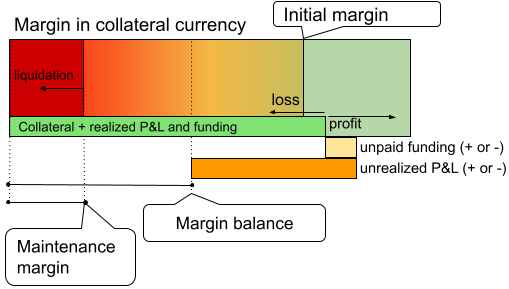
\includegraphics[width=\textwidth]{Margin.png}\\
\begin{itemize}
    \item Initial margin = position value in collateral currency * ‘initial margin rate’
    \item Margin balance = collateral + unrealized p\&l and funding
    \item Maintenance margin = position value in collateral currency * ’maintenance margin rate’
    \item Available initial margin = margin balance - initial margin
    \item Available maintenance margin = margin balance - maintenance margin
\end{itemize}






\end{textbox}

\clearpage
\section{Details}
\begin{textbox}{Margin Rates}
    \begin{itemize}
        \item initial margin rate\\
        \formula{$\tau^+ = \text{min}(\alpha_1 + \beta \cdot \text{position}, 10\%)$}
        \item maintenance margin rate \\ 
        \formula{$\tau^{*}= \text{min}(\alpha_2 + \beta \cdot \text{position}, 10\%$ $-\alpha_1+\alpha_2)$}
        \item we chose $\alpha_1=0.06$, $\alpha_2=0.04$, $\beta=0.10$
        \item a small position of 0.002 BTC can have a $\approx$16x-leverage
        (a margin rate of $0.06+0.1\cdot 0.002 \approx 0.06$)
        \item a small position of 0.002 BTC is liquidated if the margin balance drops below 4\% 
        ($0.04+0.1\cdot 0.002 \approx 0.04$), which is about 25x leverage
        \item large positions can have 10x-leverage (=10\% initial margin) and are liquidated if
        the margin balance falls below 8\% ($\approx$12x-leverage)
    \end{itemize}

\end{textbox}

\begin{textbox}{Margin balance}
    \formula{$b = \Pi( \bar{s}_2 - \bar{s})/s_3 + m_c$}
    \begin{align}
 b &: \text{margin balance in collateral currency}\\
 \bar{s}_2 &: \text{current mark price}\\
 \bar{s} &: \text{average entry price}\\
 s_3 &: \text{index price collateral currency, coll.\ to quote conversion}\\
 s_2 &: \text{index price base currency, base to quote conversion}\\
 \Pi   &: \text{trader's current position}\\
  m_c &: \text{trader collateral (in collateral currency, incl. realized P\&L)}
\end{align}
\end{textbox}

\begin{textbox}{Pricing Intuition}
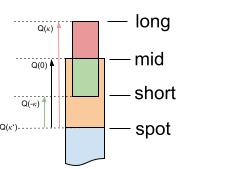
\includegraphics[width=0.75\textwidth]{pricing.png}\\
The \textbf{Mid Price} is the price of an infinitesimal small trade.
The \textbf{Spot Price} is the price of the underlying instrument provided through
an index (or oracle).
\begin{itemize}
    \item The difference between the spot price and the perpetual price
can be viewed as an \emph{insurance premium}
\item The perpetual mid-price deviation from spot, $Q(0)$, 
    corresponds to the value of the insurance that the AMM provides
\item The diagram corresponds to the situation in which the majority of the traders are long
\item Long traders further increase the risk (in this situation) and pay a price above the mid-price,
    which is not in their favor.
\item Short traders decrease
    the risk and receive a premium compared to the spot-price, which is in their favor.
\item A trade of size $\kappa^\star$ brings the AMM to minimal risk exposure,
    a situation where the insurance premium is zero and the perpetual price equals the spot.
\item If the majority of the traders are short, the mid price is below spot, and
    the insurance premium is paid by the short, received by the long
\end{itemize}
\end{textbox}

\begin{textbox}{Margin Requirement}
    \formula{$b \overset{!}{>} |\Pi| \tau \bar{s}_2/s_3$}
    \begin{align}
 b &: \text{margin balance}\\
 \tau   &: \text{targeted margin rate}\\
 s_3 &: \text{index price collateral currency, coll.\ to quote conversion}\\
 \bar{s}_2 &: \text{mark price, base to quote conversion}\\
 \Pi   &: \text{trader's current position}
\end{align}
\begin{itemize}
    \item \textbf{Current margin rate} $M = b/(|\Pi| \bar{s}_2/s_3)$\\
    \item \textbf{Liquidation} if $M < \tau^*$, where $\tau^*$ is the maintenance margin rate\\
    \item Opening trades need to fulfill the initial margin requirement
    \item \textbf{Initial Margin Requirement} $M > \tau^+$, where $\tau^+$ is the initial margin rate\\
\end{itemize}
\end{textbox}


\begin{textbox}{Leverage}
\green{Max Leverage = 1 / Initial Margin Rate}
\begin{itemize}
    \item The trader deposits a margin and can go long or short a notional
    amount that exceeds the value of the margin 
    \begin{itemize}
        \item For example, deposit 0.25 BTC
        and trade 0.5 BTC in \textbf{\color{red}{BTC}\color{mygreen}{USD} - \color{blue}{BTC}}. 
        If BTC increases from \$40,000 to \$60,000, the profit is 0.5 (\$60,000 - \$40,000) =
        \$10,000, paid in collateral currency
    \end{itemize}
    \item $Leverage = 1/ current margin rate$
    \item There is a maximal leverage specific to the perpetual, determined by the
        \emph{initial margin rate}.
\end{itemize}
\end{textbox}




%---------------------------------------------
\AtNextBibliography{\footnotesize}
\printbibliography  
\end{multicols}

\end{document}
